% Chapter 2.8: Combinational Circuits (0-OS) - LaTeX Beamer Slides
% Structured Computer Architecture: An Order-Based Approach
% Authors: John Glossner and Gheorghe M. Ştefan

\documentclass[aspectratio=169,11pt]{beamer}

% Theme and color scheme (simple, print-friendly)
\usetheme{default}
\usecolortheme{default}

% Simple color scheme for printing
\definecolor{titlecolor}{RGB}{0,0,0}
\definecolor{accentcolor}{RGB}{0,0,139}
\definecolor{textcolor}{RGB}{0,0,0}

% Set colors
\setbeamercolor{title}{fg=titlecolor}
\setbeamercolor{frametitle}{fg=titlecolor}
\setbeamercolor{structure}{fg=accentcolor}
\setbeamercolor{normal text}{fg=textcolor}

% Remove navigation symbols
\setbeamertemplate{navigation symbols}{}

% Simple footline
\setbeamertemplate{footline}[frame number]

% Packages
\usepackage{amsmath}
\usepackage{amsfonts}
\usepackage{amssymb}
\usepackage{graphicx}
\usepackage{tikz}
\usepackage{booktabs}
\usepackage{array}
\usepackage{listings}
\usepackage{xcolor}

% Set graphics path for images (relative to slides directory)
\graphicspath{{../Images/}}

% Title information
\title[Chapter 2.8: Combinational Circuits]{Structured Computer Architecture\\Chapter 2.8: Combinational Circuits\\Zero-Order Systems (0-OS)}
\subtitle{An Order-Based Approach}
\author{John Glossner and Gheorghe M. Ştefan}
\institute{Based on the textbook}
\date{\today}

% Custom commands
\newcommand{\concept}[1]{\textbf{\color{accentcolor}#1}}
\newcommand{\defterm}[1]{\textit{#1}}

\begin{document}

% Title slide
\begin{frame}
\titlepage
\end{frame}

% Table of contents
\begin{frame}{Outline}
\tableofcontents
\end{frame}

% Learning Objectives
\begin{frame}{Learning Objectives}
By the end of this chapter, you will be able to:
\begin{itemize}
\item Understand the fundamentals of Boolean algebra and its applications
\item Construct and analyze truth tables for logical operations
\item Design and optimize combinational logic circuits
\item Apply Boolean laws and identities for circuit simplification
\item Understand the relationship between mathematical logic and digital circuits
\item Recognize the historical development of Boolean algebra in computing
\end{itemize}
\end{frame}

% Section 1: Introduction to 0-OS
\section{Introduction to Zero-Order Systems}

\begin{frame}{What are Zero-Order Systems (0-OS)?}
\begin{itemize}
\item \concept{Definition}: Digital systems with \textbf{no feedback loops}
\begin{itemize}
\item Output depends \textit{only} on current input values
\item No memory or state retention
\item Purely combinational behavior
\end{itemize}
\vspace{0.5cm}
\item \concept{Characteristics}:
\begin{itemize}
\item Immediate response to input changes
\item No temporal dependencies
\item Foundation for all digital logic
\item Building blocks for higher-order systems
\end{itemize}
\vspace{0.3cm}
\item \concept{Examples}: Logic gates, decoders, multiplexers, adders
\end{itemize}
\end{frame}

\begin{frame}{Order-Based System Hierarchy}
\begin{itemize}
\item \concept{0-OS (Zero-Order)}: Combinational circuits
\begin{itemize}
\item No loops, no memory
\item Output = f(current inputs)
\end{itemize}
\vspace{0.3cm}
\item \concept{1-OS (First-Order)}: Memory circuits
\begin{itemize}
\item One feedback loop
\item Can store state
\end{itemize}
\vspace{0.3cm}
\item \concept{2-OS (Second-Order)}: Automata
\begin{itemize}
\item Two feedback loops
\item Autonomous behavior
\end{itemize}
\vspace{0.3cm}
\item \concept{3-OS (Third-Order)}: Processors
\begin{itemize}
\item Three feedback loops
\item Complex computational behavior
\end{itemize}
\end{itemize}
\end{frame}

% Section 2: Boolean Algebra
\section{Boolean Algebra}

\begin{frame}{Historical Background}
\begin{itemize}
\item \concept{George Boole (1815-1864)}:
\begin{itemize}
\item Published "An Investigation of the Laws of Thought" (1854)
\item Formalized logical reasoning using algebraic structures
\item Created symbolic language for logic
\end{itemize}
\vspace{0.5cm}
\item \concept{Claude Shannon (1916-2001)}:
\begin{itemize}
\item Master's thesis: "A Symbolic Analysis of Relay and Switching Circuits" (1938)
\item Connected Boolean algebra to electrical circuits
\item Foundation of digital circuit design
\item Enabled modern computer development
\end{itemize}
\vspace{0.3cm}
\item \concept{Impact}: Transformed abstract mathematics into practical engineering tool
\end{itemize}
\end{frame}

\begin{frame}{Boolean Algebra Fundamentals}
\begin{itemize}
\item \concept{Binary Set}: $B = \{0, 1\}$
\begin{itemize}
\item $0$ represents \textbf{false}
\item $1$ represents \textbf{true}
\end{itemize}
\vspace{0.5cm}
\item \concept{Basic Operations}:
\begin{itemize}
\item \textbf{AND} ($\land$): $A \land B = 1$ iff both $A = 1$ and $B = 1$
\item \textbf{OR} ($\lor$): $A \lor B = 1$ if at least one of $A$ or $B$ equals $1$
\item \textbf{NOT} ($\neg$): $\neg A = 1$ if $A = 0$, and $\neg A = 0$ if $A = 1$
\end{itemize}
\vspace{0.3cm}
\item \concept{Physical Interpretation}:
\begin{itemize}
\item $0$ = Low voltage, switch open, false
\item $1$ = High voltage, switch closed, true
\end{itemize}
\end{itemize}
\end{frame}

\begin{frame}{Boolean Laws and Identities}
\begin{columns}
\begin{column}{0.5\textwidth}
\concept{Commutative Laws}:
\begin{align}
A \lor B &= B \lor A\\
A \land B &= B \land A
\end{align}

\concept{Associative Laws}:
\begin{align}
A \lor (B \lor C) &= (A \lor B) \lor C\\
A \land (B \land C) &= (A \land B) \land C
\end{align}

\concept{Distributive Laws}:
\begin{align}
A \land (B \lor C) &= (A \land B) \lor (A \land C)\\
A \lor (B \land C) &= (A \lor B) \land (A \lor C)
\end{align}
\end{column}
\begin{column}{0.5\textwidth}
\concept{Identity Laws}:
\begin{align}
A \lor 0 &= A\\
A \land 1 &= A
\end{align}

\concept{Complement Laws}:
\begin{align}
A \lor \neg A &= 1\\
A \land \neg A &= 0
\end{align}

\concept{De Morgan's Laws}:
\begin{align}
\neg(A \lor B) &= \neg A \land \neg B\\
\neg(A \land B) &= \neg A \lor \neg B
\end{align}
\end{column}
\end{columns}
\end{frame}

\begin{frame}{Boolean Algebra Applications}
\begin{itemize}
\item \concept{Circuit Simplification}:
\begin{itemize}
\item Reduce number of gates required
\item Minimize cost and complexity
\item Improve performance and reliability
\end{itemize}
\vspace{0.5cm}
\item \concept{Simplification Methods}:
\begin{itemize}
\item \textbf{Boolean identities}: Algebraic manipulation
\item \textbf{Karnaugh maps}: Graphical simplification method
\item \textbf{Quine-McCluskey algorithm}: Tabular minimization approach
\end{itemize}
\vspace{0.5cm}
\item \concept{Logic Conversion}:
\begin{itemize}
\item Convert between AND-OR and NAND-NOR logic
\item Transform to preferred gate types
\item Optimize for specific technologies
\end{itemize}
\end{itemize}
\end{frame}

% Section 3: Truth Tables
\section{Truth Tables}

\begin{frame}{Truth Table Fundamentals}
\begin{itemize}
\item \concept{Definition}: Systematic representation of logical expressions
\begin{itemize}
\item Lists all possible input combinations
\item Shows corresponding output values
\item Complete behavioral specification
\end{itemize}
\vspace{0.5cm}
\item \concept{Structure Components}:
\begin{itemize}
\item \textbf{Input Variables}: Columns for logical variables ($A, B, \ldots, N$)
\item \textbf{Output Values}: Results of logical operations
\item \textbf{Rows}: $2^n$ combinations for $n$ variables
\end{itemize}
\vspace{0.3cm}
\item \concept{Applications}:
\begin{itemize}
\item Circuit analysis and design
\item Logic verification
\item Boolean function specification
\end{itemize}
\end{itemize}
\end{frame}

\begin{frame}{Basic Logic Operations - Truth Tables}
\begin{columns}
\begin{column}{0.25\textwidth}
\concept{NOT Operation}:
\[
\begin{array}{|c|c|}
\hline
A & \neg A \\
\hline
0 & 1 \\
1 & 0 \\
\hline
\end{array}
\]
\end{column}
\begin{column}{0.35\textwidth}
\concept{AND Operation}:
\[
\begin{array}{|c|c|c|}
\hline
A & B & A \land B \\
\hline
0 & 0 & 0 \\
0 & 1 & 0 \\
1 & 0 & 0 \\
1 & 1 & 1 \\
\hline
\end{array}
\]
\end{column}
\begin{column}{0.35\textwidth}
\concept{OR Operation}:
\[
\begin{array}{|c|c|c|}
\hline
A & B & A \lor B \\
\hline
0 & 0 & 0 \\
0 & 1 & 1 \\
1 & 0 & 1 \\
1 & 1 & 1 \\
\hline
\end{array}
\]
\end{column}
\end{columns}

\vspace{0.5cm}
\begin{columns}
\begin{column}{0.5\textwidth}
\concept{XOR (Exclusive OR)}:
\[
\begin{array}{|c|c|c|}
\hline
A & B & A \oplus B \\
\hline
0 & 0 & 0 \\
0 & 1 & 1 \\
1 & 0 & 1 \\
1 & 1 & 0 \\
\hline
\end{array}
\]
\end{column}
\begin{column}{0.5\textwidth}
\concept{NAND (NOT AND)}:
\[
\begin{array}{|c|c|c|}
\hline
A & B & \neg(A \land B) \\
\hline
0 & 0 & 1 \\
0 & 1 & 1 \\
1 & 0 & 1 \\
1 & 1 & 0 \\
\hline
\end{array}
\]
\end{column}
\end{columns}
\end{frame}

\begin{frame}{Advanced Logic Operations}
\begin{columns}
\begin{column}{0.5\textwidth}
\concept{NOR (NOT OR)}:
\[
\begin{array}{|c|c|c|}
\hline
A & B & \neg(A \lor B) \\
\hline
0 & 0 & 1 \\
0 & 1 & 0 \\
1 & 0 & 0 \\
1 & 1 & 0 \\
\hline
\end{array}
\]
\end{column}
\begin{column}{0.5\textwidth}
\concept{XNOR (Equivalence)}:
\[
\begin{array}{|c|c|c|}
\hline
A & B & A \odot B \\
\hline
0 & 0 & 1 \\
0 & 1 & 0 \\
1 & 0 & 0 \\
1 & 1 & 1 \\
\hline
\end{array}
\]
\end{column}
\end{columns}

\vspace{0.5cm}
\concept{Key Properties}:
\begin{itemize}
\item \textbf{NAND}: Universal gate (can implement any Boolean function)
\item \textbf{NOR}: Also universal gate
\item \textbf{XOR}: Useful for parity checking and arithmetic
\item \textbf{XNOR}: Equivalence testing and error detection
\end{itemize}
\end{frame}

\begin{frame}{Truth Table Applications}
\begin{itemize}
\item \concept{Circuit Analysis}:
\begin{itemize}
\item Verify circuit behavior
\item Compare expected vs. actual outputs
\item Debug logic errors
\end{itemize}
\vspace{0.5cm}
\item \concept{Function Specification}:
\begin{itemize}
\item Define required circuit behavior
\item Specify input-output relationships
\item Document design requirements
\end{itemize}
\vspace{0.5cm}
\item \concept{Logic Synthesis}:
\begin{itemize}
\item Convert truth tables to Boolean expressions
\item Generate minimal circuit implementations
\item Optimize for area, speed, or power
\end{itemize}
\end{itemize}
\end{frame}

% Section 4: Logic Gates and Circuits
\section{Logic Gates and Digital Circuits}

\begin{frame}{Physical Implementation of Logic Gates}
\begin{itemize}
\item \concept{Transistor-Level Implementation}:
\begin{itemize}
\item CMOS technology (Complementary Metal-Oxide-Semiconductor)
\item NMOS and PMOS transistors
\item Low power consumption and high noise immunity
\end{itemize}
\vspace{0.5cm}
\item \concept{Gate Characteristics}:
\begin{itemize}
\item \textbf{Propagation delay}: Time for output to respond to input change
\item \textbf{Fan-in}: Number of inputs a gate can accept
\item \textbf{Fan-out}: Number of gates an output can drive
\item \textbf{Noise margin}: Tolerance to signal variations
\end{itemize}
\vspace{0.3cm}
\item \concept{Performance Considerations}:
\begin{itemize}
\item Speed vs. power trade-offs
\item Area optimization
\item Signal integrity
\end{itemize}
\end{itemize}
\end{frame}

\begin{frame}{Combinational Circuit Design Process}
\begin{enumerate}
\item \concept{Problem Specification}:
\begin{itemize}
\item Define input and output requirements
\item Specify functional behavior
\item Identify constraints (timing, power, area)
\end{itemize}
\vspace{0.3cm}
\item \concept{Truth Table Construction}:
\begin{itemize}
\item List all input combinations
\item Determine corresponding outputs
\item Verify completeness and correctness
\end{itemize}
\vspace{0.3cm}
\item \concept{Boolean Expression Derivation}:
\begin{itemize}
\item Sum-of-products (SOP) form
\item Product-of-sums (POS) form
\item Choose optimal representation
\end{itemize}
\vspace{0.3cm}
\item \concept{Circuit Implementation}:
\begin{itemize}
\item Select appropriate gates
\item Optimize for design goals
\item Verify functionality
\end{itemize}
\end{enumerate}
\end{frame}

\begin{frame}{Half Adder Circuit}
\begin{columns}
\begin{column}{0.6\textwidth}
\concept{Function}: Adds two single bits
\begin{itemize}
\item Inputs: $A$, $B$
\item Outputs: Sum ($S$), Carry ($C$)
\end{itemize}

\vspace{0.3cm}
\concept{Truth Table}:
\[
\begin{array}{|c|c|c|c|}
\hline
A & B & S & C \\
\hline
0 & 0 & 0 & 0 \\
0 & 1 & 1 & 0 \\
1 & 0 & 1 & 0 \\
1 & 1 & 0 & 1 \\
\hline
\end{array}
\]

\vspace{0.3cm}
\concept{Boolean Expressions}:
\begin{align}
S &= A \oplus B\\
C &= A \land B
\end{align}
\end{column}
\begin{column}{0.4\textwidth}
\begin{center}
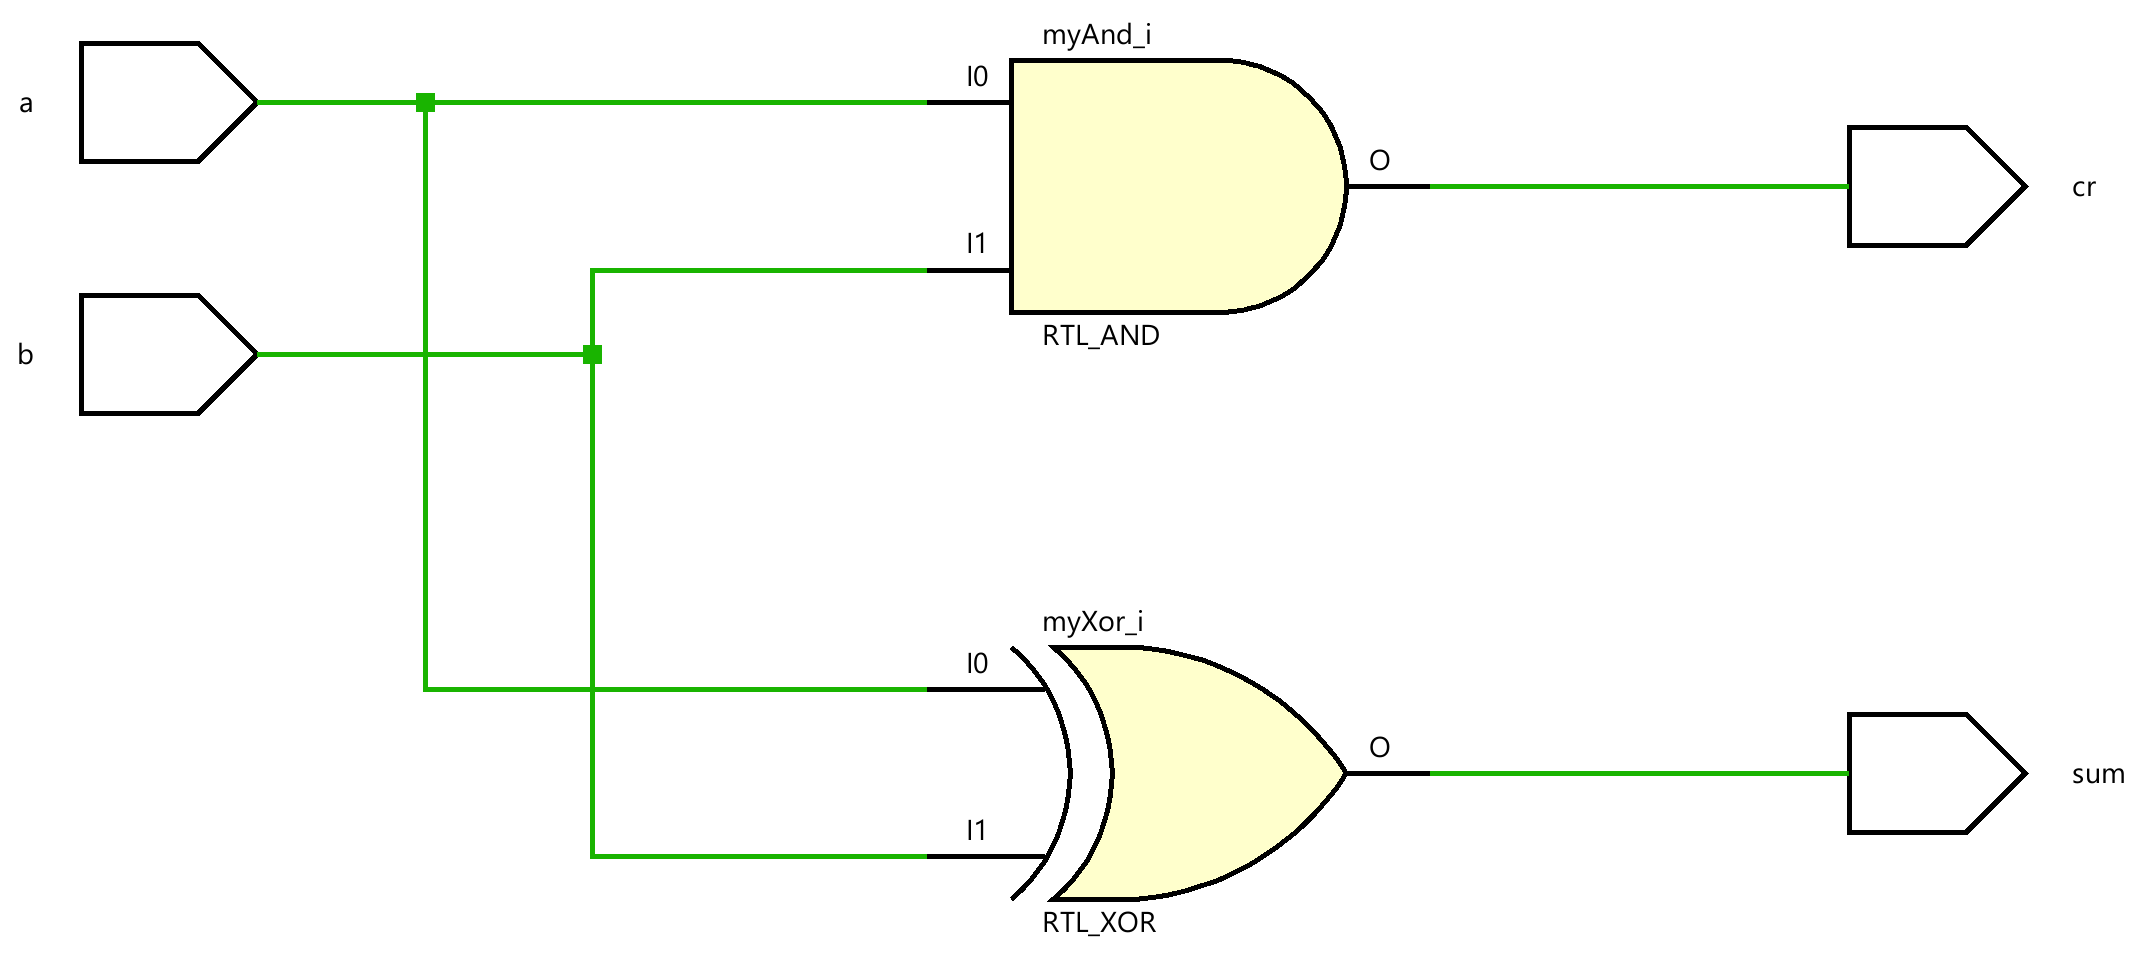
\includegraphics[width=\textwidth]{halfAdder.png}
\end{center}
\concept{Implementation}:
\begin{itemize}
\item XOR gate for sum
\item AND gate for carry
\item Fundamental building block
\end{itemize}
\end{column}
\end{columns}
\end{frame}

\begin{frame}{Full Adder Circuit}
\begin{columns}
\begin{column}{0.6\textwidth}
\concept{Function}: Adds three bits (including carry-in)
\begin{itemize}
\item Inputs: $A$, $B$, $C_{in}$
\item Outputs: Sum ($S$), Carry-out ($C_{out}$)
\end{itemize}

\vspace{0.3cm}
\concept{Truth Table}:
\[
\begin{array}{|c|c|c|c|c|}
\hline
A & B & C_{in} & S & C_{out} \\
\hline
0 & 0 & 0 & 0 & 0 \\
0 & 0 & 1 & 1 & 0 \\
0 & 1 & 0 & 1 & 0 \\
0 & 1 & 1 & 0 & 1 \\
1 & 0 & 0 & 1 & 0 \\
1 & 0 & 1 & 0 & 1 \\
1 & 1 & 0 & 0 & 1 \\
1 & 1 & 1 & 1 & 1 \\
\hline
\end{array}
\]
\end{column}
\begin{column}{0.4\textwidth}
\begin{center}
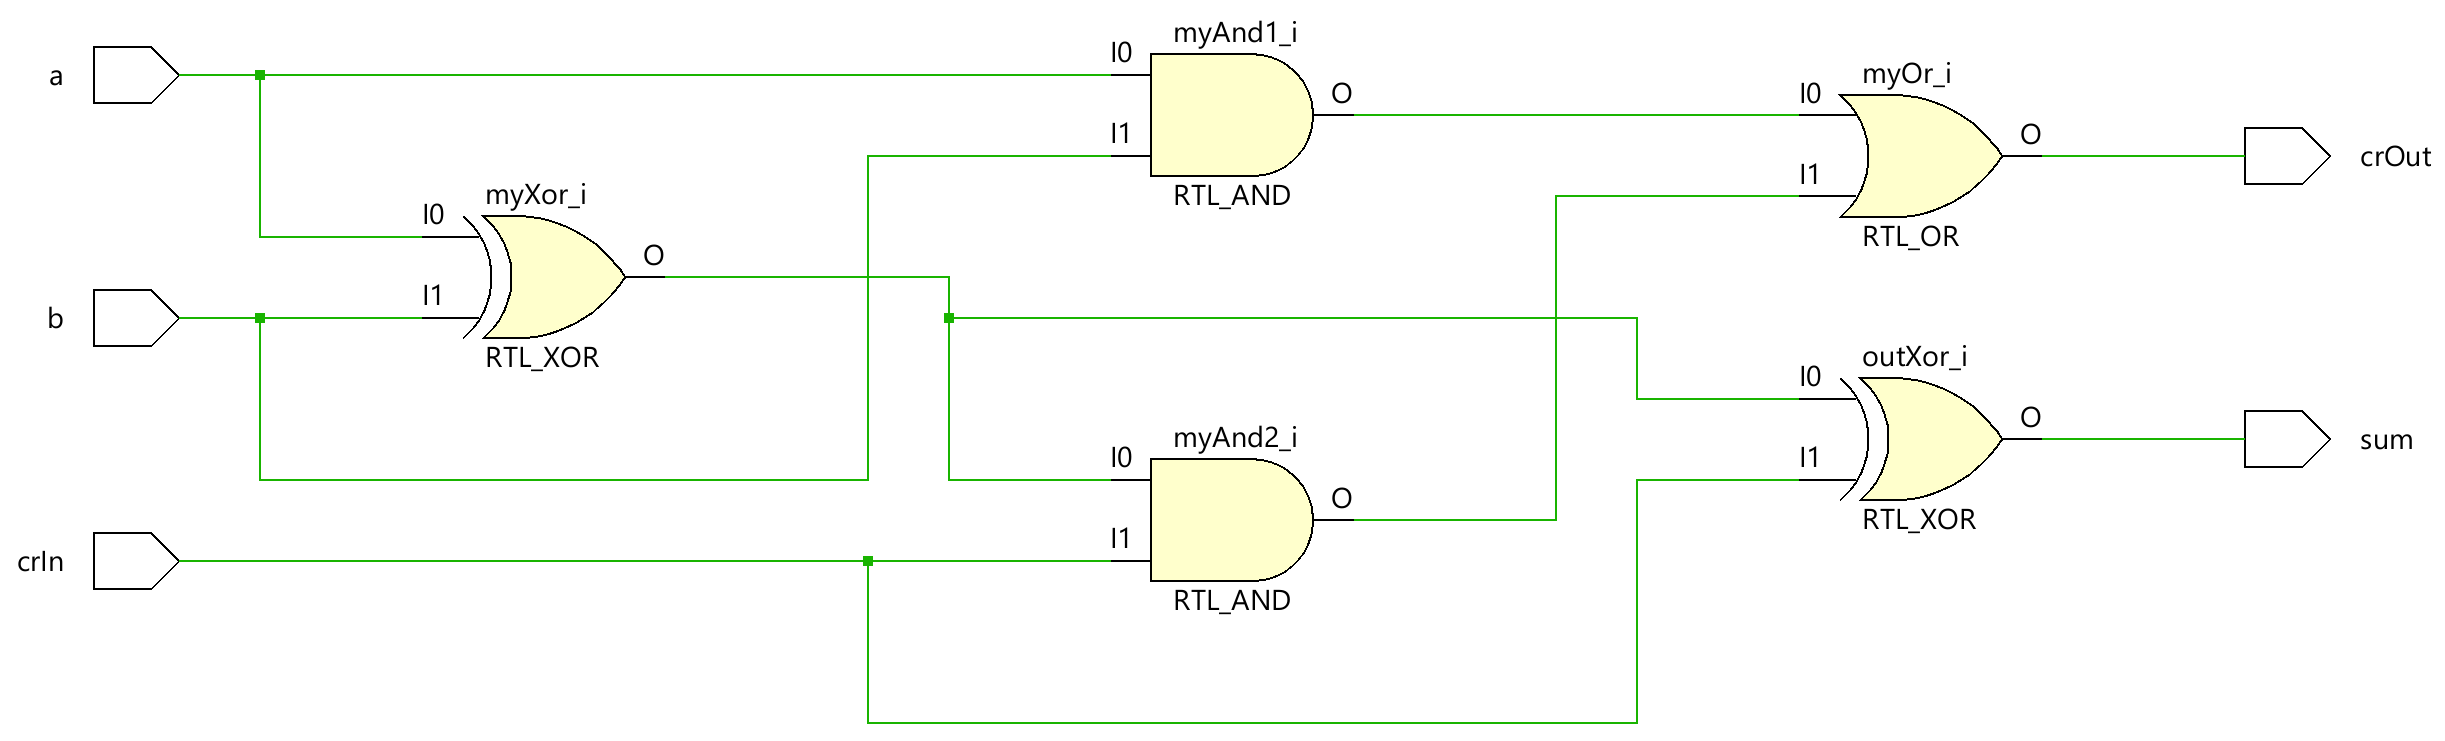
\includegraphics[width=\textwidth]{fullAdder.png}
\end{center}
\concept{Boolean Expressions}:
\begin{align}
S &= A \oplus B \oplus C_{in}\\
C_{out} &= AB + C_{in}(A \oplus B)
\end{align}
\end{column}
\end{columns}
\end{frame}

% Section 5: Combinational Building Blocks
\section{Combinational Building Blocks}

\begin{frame}{Decoders}
\begin{itemize}
\item \concept{Function}: Convert binary code to one-hot output
\begin{itemize}
\item $n$ inputs produce $2^n$ outputs
\item Only one output is active (high) at a time
\item Used for address decoding and selection
\end{itemize}
\vspace{0.5cm}
\item \concept{2-to-4 Decoder Example}:
\begin{itemize}
\item Inputs: $A_1$, $A_0$
\item Outputs: $Y_0$, $Y_1$, $Y_2$, $Y_3$
\item $Y_i = 1$ when input equals $i$ in binary
\end{itemize}
\vspace{0.3cm}
\item \concept{Applications}:
\begin{itemize}
\item Memory address decoding
\item Instruction decoding in processors
\item Device selection in systems
\item Seven-segment display drivers
\end{itemize}
\end{itemize}
\end{frame}

\begin{frame}{Multiplexers (Data Selectors)}
\begin{itemize}
\item \concept{Function}: Select one of multiple inputs based on control signals
\begin{itemize}
\item $2^n$ data inputs, $n$ select inputs
\item One output that equals selected input
\item Digital equivalent of rotary switch
\end{itemize}
\vspace{0.5cm}
\item \concept{4-to-1 Multiplexer}:
\begin{itemize}
\item Data inputs: $D_0$, $D_1$, $D_2$, $D_3$
\item Select inputs: $S_1$, $S_0$
\item Output: $Y = D_i$ where $i = S_1S_0$
\end{itemize}
\vspace{0.3cm}
\item \concept{Applications}:
\begin{itemize}
\item Data routing and switching
\item Function generation
\item Parallel-to-serial conversion
\item Processor data paths
\end{itemize}
\end{itemize}
\end{frame}

\begin{frame}{Demultiplexers (Data Distributors)}
\begin{itemize}
\item \concept{Function}: Route single input to one of multiple outputs
\begin{itemize}
\item One data input, $n$ select inputs
\item $2^n$ outputs, only one receives data
\item Inverse operation of multiplexer
\end{itemize}
\vspace{0.5cm}
\item \concept{1-to-4 Demultiplexer}:
\begin{itemize}
\item Data input: $D$
\item Select inputs: $S_1$, $S_0$
\item Outputs: $Y_0$, $Y_1$, $Y_2$, $Y_3$
\item $Y_i = D$ when $i = S_1S_0$, others = 0
\end{itemize}
\vspace{0.3cm}
\item \concept{Applications}:
\begin{itemize}
\item Data distribution
\item Serial-to-parallel conversion
\item Address decoding with enable
\item Communication systems
\end{itemize}
\end{itemize}
\end{frame}

\begin{frame}{Encoders}
\begin{itemize}
\item \concept{Function}: Convert one-hot input to binary code
\begin{itemize}
\item $2^n$ inputs produce $n$ outputs
\item Inverse operation of decoder
\item Assumes only one input is active
\end{itemize}
\vspace{0.5cm}
\item \concept{Priority Encoder}:
\begin{itemize}
\item Handles multiple active inputs
\item Encodes highest priority input
\item Includes valid output signal
\item More practical than simple encoder
\end{itemize}
\vspace{0.3cm}
\item \concept{Applications}:
\begin{itemize}
\item Keyboard encoding
\item Interrupt priority encoding
\item Data compression
\item Position encoding
\end{itemize}
\end{itemize}
\end{frame}

% Section 6: Circuit Optimization
\section{Circuit Optimization and Minimization}

\begin{frame}{Karnaugh Maps (K-Maps)}
\begin{itemize}
\item \concept{Purpose}: Graphical method for Boolean function minimization
\begin{itemize}
\item Visual representation of truth table
\item Adjacent cells differ by one variable
\item Groups of 1s indicate simplified terms
\end{itemize}
\vspace{0.5cm}
\item \concept{Procedure}:
\begin{enumerate}
\item Plot function on K-map grid
\item Identify groups of adjacent 1s
\item Groups must be powers of 2 (1, 2, 4, 8, ...)
\item Write simplified expression from groups
\end{enumerate}
\vspace{0.3cm}
\item \concept{Advantages}:
\begin{itemize}
\item Intuitive visual approach
\item Guaranteed minimal result for small functions
\item Easy to identify don't-care conditions
\end{itemize}
\end{itemize}
\end{frame}

\begin{frame}{Quine-McCluskey Algorithm}
\begin{itemize}
\item \concept{Purpose}: Systematic tabular minimization method
\begin{itemize}
\item Algorithmic approach to Boolean minimization
\item Handles any number of variables
\item Computer-implementable procedure
\end{itemize}
\vspace{0.5cm}
\item \concept{Steps}:
\begin{enumerate}
\item List all minterms in binary
\item Find prime implicants by combining terms
\item Construct prime implicant table
\item Select minimal set of prime implicants
\end{enumerate}
\vspace{0.3cm}
\item \concept{Advantages}:
\begin{itemize}
\item Systematic and complete
\item Handles large numbers of variables
\item Suitable for computer automation
\item Finds all minimal solutions
\end{itemize}
\end{itemize}
\end{frame}

\begin{frame}{Design Optimization Goals}
\begin{itemize}
\item \concept{Area Minimization}:
\begin{itemize}
\item Reduce number of gates
\item Minimize chip area and cost
\item Important for high-volume production
\end{itemize}
\vspace{0.3cm}
\item \concept{Speed Optimization}:
\begin{itemize}
\item Minimize propagation delay
\item Reduce critical path length
\item May require more gates for parallelism
\end{itemize}
\vspace{0.3cm}
\item \concept{Power Minimization}:
\begin{itemize}
\item Reduce switching activity
\item Use low-power gate designs
\item Critical for mobile and embedded systems
\end{itemize}
\vspace{0.3cm}
\item \concept{Trade-offs}:
\begin{itemize}
\item Speed vs. area vs. power
\item Design constraints determine priorities
\item Technology-dependent optimizations
\end{itemize}
\end{itemize}
\end{frame}

% Section 7: Advanced Topics
\section{Advanced Combinational Concepts}

\begin{frame}{Hazards and Glitches}
\begin{itemize}
\item \concept{Static Hazards}:
\begin{itemize}
\item Output momentarily changes when it should remain constant
\item Caused by unequal propagation delays
\item Can be eliminated by adding redundant terms
\end{itemize}
\vspace{0.5cm}
\item \concept{Dynamic Hazards}:
\begin{itemize}
\item Output changes multiple times during transition
\item More complex to analyze and eliminate
\item Usually avoided through careful design
\end{itemize}
\vspace{0.5cm}
\item \concept{Prevention Techniques}:
\begin{itemize}
\item Add consensus terms to cover hazards
\item Use synchronous design methodology
\item Careful timing analysis and verification
\item Buffer insertion for delay matching
\end{itemize}
\end{itemize}
\end{frame}

\begin{frame}{Technology Mapping}
\begin{itemize}
\item \concept{Gate Library Constraints}:
\begin{itemize}
\item Available gates in target technology
\item Drive strength and loading considerations
\item Area and delay characteristics
\end{itemize}
\vspace{0.5cm}
\item \concept{NAND/NOR Implementation}:
\begin{itemize}
\item Universal gates can implement any function
\item Often preferred in CMOS technology
\item Requires function transformation
\end{itemize}
\vspace{0.5cm}
\item \concept{Optimization Considerations}:
\begin{itemize}
\item Technology-specific optimizations
\item Wire delay vs. gate delay
\item Power and thermal constraints
\item Manufacturing yield considerations
\end{itemize}
\end{itemize}
\end{frame}

\begin{frame}{Arithmetic Circuits}
\begin{itemize}
\item \concept{Multi-bit Adders}:
\begin{itemize}
\item Ripple-carry adder: Simple but slow
\item Carry-lookahead adder: Faster but more complex
\item Carry-select adder: Speed-area trade-off
\end{itemize}
\vspace{0.5cm}
\item \concept{Subtraction Circuits}:
\begin{itemize}
\item Two's complement representation
\item Subtraction as addition of complement
\item Overflow detection logic
\end{itemize}
\vspace{0.5cm}
\item \concept{Comparison Circuits}:
\begin{itemize}
\item Magnitude comparators
\item Equality detection
\item Greater-than/less-than logic
\end{itemize}
\end{itemize}
\end{frame}

% Section 8: Summary
\section{Chapter Summary}

\begin{frame}{Key Concepts Review}
\begin{itemize}
\item \concept{Boolean Algebra Foundations}:
\begin{itemize}
\item Mathematical basis for digital logic
\item Laws and identities for simplification
\item Historical development from Boole to Shannon
\end{itemize}
\vspace{0.3cm}
\item \concept{Truth Tables and Logic Operations}:
\begin{itemize}
\item Systematic representation of logical functions
\item Basic and advanced logic operations
\item Circuit analysis and verification tool
\end{itemize}
\vspace{0.3cm}
\item \concept{Combinational Circuit Design}:
\begin{itemize}
\item Systematic design methodology
\item Building blocks: decoders, multiplexers, adders
\item Optimization techniques and trade-offs
\end{itemize}
\end{itemize}
\end{frame}

\begin{frame}{Practical Applications}
\begin{itemize}
\item \concept{Digital System Building Blocks}:
\begin{itemize}
\item Foundation for all digital circuits
\item Essential components in processors
\item Building blocks for memory systems
\end{itemize}
\vspace{0.3cm}
\item \concept{Design Methodology}:
\begin{itemize}
\item Specification to implementation flow
\item Optimization for different goals
\item Verification and testing approaches
\end{itemize}
\vspace{0.3cm}
\item \concept{Technology Considerations}:
\begin{itemize}
\item Physical implementation constraints
\item Performance optimization techniques
\item Power and area trade-offs
\end{itemize}
\end{itemize}
\end{frame}

\begin{frame}{Connection to Higher-Order Systems}
\begin{itemize}
\item \concept{Foundation for 1-OS (Memory Circuits)}:
\begin{itemize}
\item Combinational logic + feedback = memory
\item State storage and retention
\item Clocking and synchronization
\end{itemize}
\vspace{0.3cm}
\item \concept{Building Blocks for 2-OS (Automata)}:
\begin{itemize}
\item Control logic implementation
\item State transition logic
\item Output generation circuits
\end{itemize}
\vspace{0.3cm}
\item \concept{Components of 3-OS (Processors)}:
\begin{itemize}
\item Arithmetic and logic units
\item Instruction decoding logic
\item Data path components
\end{itemize}
\end{itemize}
\end{frame}

% Questions slide
\begin{frame}{Questions and Discussion}
\begin{center}
\Large
Questions?

\vspace{1cm}

\normalsize
\textbf{Discussion Topics:}
\begin{itemize}
\item How do Boolean laws enable circuit optimization?
\item What are the trade-offs between different adder architectures?
\item Why are NAND and NOR gates considered universal?
\item How do combinational circuits form the foundation for sequential systems?
\end{itemize}

\vspace{0.5cm}
\textbf{Next:} Chapter 2.9 - Memory Circuits: First-Order Systems (1-OS)
\end{center}
\end{frame}

\end{document}

